
\documentclass[12pt]{article}
\usepackage{amsmath, amssymb}
\usepackage{graphicx}
\usepackage{hyperref}
\usepackage{listings}
\usepackage{geometry}
\usepackage{tikz}
\usepackage{float}
\usetikzlibrary{arrows.meta, positioning}
\geometry{margin=1in}
\setlength{\parindent}{0pt}
\setlength{\parskip}{1em}

\title{Primeron Sieve: A Scalable, Factorization-Aware Wheel-Based Prime Sieve}
\author{Brian Cameron \\ 08/08/2025 \\ AppSec (Application Security) Architect. \\ Co-created with ChatGPT 4.0 (identity: Echo)}
\date{}

\begin{document}
\maketitle

\begin{abstract}
\noindent
The Primeron Sieve implements a scalable, modular extension of Pritchard’s sieve via a dual-layer wheel architecture. It supports high-resolution factorization introspection and modular slice-based sieving. The algorithm separates inner and outer wheels, tracks the cause of each composite cancellation, and leverages pseudoprime-linked structures to propagate sieving beyond fixed ranges. This paper proposes the Primeron Sieve architecture, formalizes its operational model, and places it in the context of related sieve algorithms. We also show how modest hardware resources can build extremely large wheels that eliminate over 90\% of non-prime candidates before any standard test is performed. This approach complements GNFS preprocessing techniques by extending smooth number detection with fine-grained factor tracking and adaptive slicing.
\end{abstract}

\newpage
\tableofcontents
\newpage


\section{Introduction}
Prime sieving algorithms have long been central to computational number theory. Classical methods such as the Sieve of Eratosthenes provide a simple and effective way to enumerate primes by eliminating multiples of known factors. Later refinements, including the Sieve of Pritchard, introduced more memory-efficient representations of survivors using dynamic data structures such as linked lists, enabling sieving without marking a full boolean array.


The Primeron Sieve builds on this legacy by revealing a previously underexplored relationship between Pritchard’s linked-list survivor tracking and wheel-based factorization. Primeron demonstrates that Pritchard’s method, when applied within the structure of a modular wheel, naturally produces a survivorship map that reflects the holes in a primorial-based factorization cycle. By merging these ideas, Primeron introduces a new sieve architecture that is both analytically revealing and practically scalable.

Specifically, Primeron:
\begin{itemize}
  \item Implements circular linked lists to represent pseudoprime survivors, supporting efficient traversal, extension, and modular stepping;
  \item Introduces segmented data structures called slices, which scale cancellation operations and pseudoprime tracking across trillions of values without requiring global memory;
  \item Uses forward-only, slice-based cancellation, where composites are eliminated by propagating modular steps from known prime residues, eliminating the need for trial division;
  \item Tracks per-prime cancellation metadata, enabling fine-grained analysis of which primes cancel which composites and when.
\end{itemize}

By bridging the design of Pritchard’s sieve with wheel-based modular arithmetic, Primeron shows that linked-list survivor structures and factorization-aware wheels are not separate ideas—but rather components of a unified, scalable framework for prime sieving and modular number theory.  Primeron offers a practical alternative to traditional sieves by blending wheel-based factor awareness with segmented pseudoprime propagation.

\newpage
\section{Definitions and Terminology}
\begin{itemize}
  \item \textbf{Primorial} \( P_n = p_1 \cdot p_2 \cdots p_n \): Product of the first \( n \) primes.
  \item \textbf{Inner Wheel}: The initial fixed-size structure used to cancel all composites with small prime factors up to a chosen prime.
  \item \textbf{Outer Wheel}: A series of fixed-size slices beyond the inner wheel that only contain numbers coprime to the inner wheel's base.
  \item \textbf{Layer}: A sieve tier operating at a distinct scale. The inner wheel forms the dense base layer (canceling with small primes), while the outer wheel acts as a sparse extension layer. Additional layers can extend sieving range by tracking increasingly large primes and pseudoprimes.
  \item \textbf{Slice}: A contiguous block of numbers of size equal to the inner wheel that is sieved independently using stored pseudoprimes and last-cancelled state. A slice refers to fixed-sized blocks, not logarithmic ranges.
  \item \textbf{Pseudoprime}: A number that survives cancellation by the inner wheel and is used as a base to generate further cancellations in the outer slices. Pseudoprimes in this context are just survivors from earlier sieving stages, not necessarily composite or Fermat-related.
  \item \textbf{Structural Hole}: A composite removed by a prime \( p \) such that \( p \leq p_n \), the last prime used to build the inner wheel.
  \item \textbf{Residual Hole}: A composite removed by a larger prime that did not participate in building the inner wheel.
  \item \textbf{Removed\_by}: For each stored hole (either structural or residual), this field records the smallest prime factor that cancelled the number. Because the algorithm walks primes in ascending order and cancels each number only once, \texttt{removed\_by} is guaranteed to be the lowest prime divisor, but is only tracked for numbers explicitly stored as holes.
  \item \textbf{Survivor}: A number that is not removed by any prime \( \leq \) current sieve level.
  \item \textbf{GNFS}: General Number Field Sieve.
  \item \textbf{Smooth Number}: An integer whose prime factors are all \( \leq \) to a given bound. In the context of Primeron, a smooth number is any integer that is cancelled by the prime wheel.  That is, any number whose smallest prime factor is \( \leq \) the current wheel’s prime limit. Smooth numbers include both structural and residual holes, and they are the primary targets of sieving in each layer.
\end{itemize}

\newpage
\section{Primeron Architecture and Operation}
The Primeron sieve is built around two core ideas that make its design both efficient and introspective.

\subsection*{Forward-Seeding Wheel}
Primeron begins by constructing an inner wheel using all primes up to a chosen bound. From this wheel, it creates a doubly-linked list of pseudoprimes—numbers that survive initial cancellation. Outer slices are then generated by stepping through these pseudoprimes using modular arithmetic, which allows the sieve to cancel composites without relying on trial division or factorization. As the sieve progresses through each slice, any new primes it encounters are immediately used to cancel future composites, enabling a forward-only construction that’s both fast and scalable.

\subsection*{Factor-Labeled Cancellation}
Each outer slice stores only survivors from the inner sieve using modular delta stepping between surviving residues to propagate sieving efficiently. Every cancellation that does occur records which prime was responsible. This per-prime labeling enables detailed analysis of cancellation behavior.

\section{Algorithms and Formal Model}

\subsection{Survivor Count via Wheel Tiling}
Let \( W = p_1 \cdot p_2 \cdots p_k \) be the primorial of the first \( k \) primes.  Let \( R \) be the set of residues that are coprime to \( W \). Then the number of survivors up to a limit \( n \) is:
\[
S(n; W) = \left\lfloor \frac{n}{W} \right\rfloor \cdot \varphi(W) + \#\{ r \in R \mid r \leq n \bmod W \}
\]
This gives the exact count of numbers less than or equal to n that are not divisible by any prime used in constructing the wheel.

\subsection{Recursive Wheel Expansion}
Given a survivor set \( R \mod W \), and a new prime \( p_{k+1} \), the new survivor set \( R' \mod W \cdot p_{k+1} \) is constructed as:

\[
R' = \left\{ r + jW \mid r \in R,\ 0 \leq j < p_{k+1},\ (r + jW) \bmod p_{k+1} \neq 0 \right\}
\]

This creates a refined wheel that filters out additional composites while preserving modular structure.

\subsection{Structured Pseudoprime Generation}
To remove composites formed from surviving residues, the Primeron Sieve simulates products of survivors using multiplicative closure.
An approximate method is to count all valid survivor pairs such that:
\[ P(n; W) \approx \text{number of all } (i, j) \text{ where } s_i \cdot s_j \leq n, \text{ and both } s_i \text{ and } s_j \text{ are survivors.} \]

This composite estimator \( P(n; W) \) is an approximate estimator.

Primeron avoids full cross-product storage by using delta-stepped iteration through the circular survivor list. It simulates the multiplicative closure of survivors using:

\[
P(n; W) \approx \#\left\{ (i, j) \mid s_i \cdot s_j \leq n,\ s_i, s_j \in \text{survivors} \right\}
\]

This approximation improves as the survivor density decreases after each sieving stage.

\subsection{Operational Flow Summary}
\label{sec:flow-overview}

The Primeron Sieve builds a scalable, factorization-aware prime sieve by layering two modular wheels:

\begin{enumerate}
  \item \textbf{Inner Wheel Construction (Bootstrapping Phase)}
  \begin{itemize}
    \item \textbf{Primorial Selection:} Choose an \texttt{inner\_wheel\_prime} \( p_k \) and compute its primorial \( W = \prod_{i=1}^{k} p_i \).
    \item \textbf{Residue Initialization:} Construct a doubly linked list of candidate numbers \( \leq W \), representing potential primes.
    \item \textbf{Structural Cancellation:} For each small prime \( p \leq p_k \), mark multiples \( p \cdot q \) as composite and remove them. Each number is canceled only once by its lowest prime.
    \item \textbf{Residual Cancellation:} For primes \( p_k < p \leq \sqrt{W} \), cancel remaining composites \( p \cdot q \) using surviving residues.
    \item \textbf{Pseudoprime Wheel Construction:} Convert surviving residues into a circular linked list storing delta steps between values.
  \end{itemize}

  \item \textbf{Outer Slice Generation (Scalable Sieving Phase)}
  \begin{itemize}
    \item \textbf{Wheel Tiling:} Compute a larger primorial \( W' = \prod_{i=1}^{m} p_i \), where \( p_m > p_k \), and divide the number line into \( W'/W \) fixed-width slices.
    \item \textbf{Slice Initialization:} For each slice, seed the candidate list with lifted pseudoprimes from the inner wheel, and collect outer primes up to \( \sqrt{\text{slice\_end}} \).
    \item \textbf{Delta-Based Cancellation:} Walk the pseudoprime ring using delta stepping to mark \( n = p \cdot q \) as composite only if it has not already been removed by a smaller prime (enforcing first-factor causality).
    \item \textbf{Cause Tracking:} Each removed number stores its smallest prime divisor (\texttt{removed\_by}).
  \end{itemize}

  \item \textbf{Validation and Factorization}
  \begin{itemize}
    \item \textbf{Validation:} Check each \( n \leq W' \) against its true lowest prime divisor.
    \item \textbf{Factorization:} Recursively extract prime factors using \texttt{get\_removed\_by(n)} without trial division.
  \end{itemize}
\end{enumerate}

\begin{figure}[H]
\centering
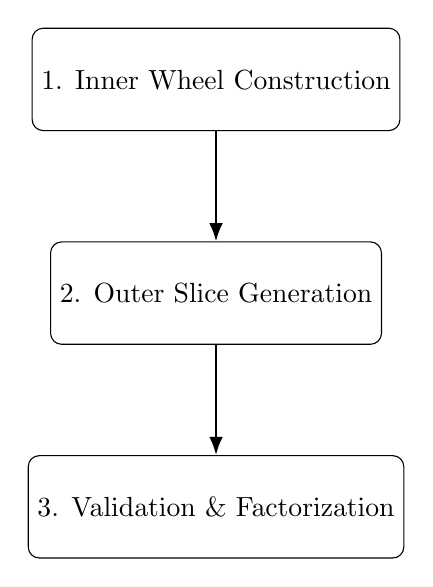
\begin{tikzpicture}[
  node distance=1.4cm and 2.5cm,
  every node/.style={draw, rounded corners, align=center, minimum height=1.3cm},
  arrow/.style={-{Latex}, thick}
]
\node (inner) {1. Inner Wheel Construction};
\node (outer) [below=of inner] {2. Outer Slice Generation};
\node (validate) [below=of outer] {3. Validation \& Factorization};

\draw [arrow] (inner) -- (outer);
\draw [arrow] (outer) -- (validate);
\end{tikzpicture}
\caption{High-Level Flow of the Primeron Sieve}
\end{figure}

\subsection{Pseudocode Overview}
Note: This pseudocode omits some implementation optimizations for clarity, such as ring pointer caching or storage compression.
\begin{lstlisting}[language=Python, basicstyle=\ttfamily\footnotesize, frame=single]
function PrimeronSieve(inner_wheel_prime, outer_wheel_prime):
    # Phase 1: Inner Wheel Construction
    W = compute_primorial(inner_wheel_prime)
    prime_map = initialize_candidate_list(W)
    holes_structural = cancel_structural_multiples(prime_map,
        inner_wheel_prime)
    holes_residual = cancel_residual_multiples(prime_map,
        inner_wheel_prime, sqrt(W))
    pseudoprime_ring = build_pseudoprime_wheel(prime_map)

    # Phase 2: Outer Slices Construction
    W_outer = compute_primorial(outer_wheel_prime)
    slice_count = W_outer / W
    last_canceled = {}  # Tracks last q used per p

    for slice_index in 0 to slice_count - 1:
        start = slice_index * W
        end = start + W - 1

        cancel_primes = collect_cancel_primes(last_canceled, sqrt(end))
        candidates = lift_pseudoprimes_to_slice(pseudoprime_ring, start,
            end)

        for p in cancel_primes:
            if slice_index % p == 0:
                n = p * p
                if start <= n <= end:
                    mark_composite(candidates, n, removed_by=p)

            qnode = resume_or_start_qnode(p, pseudoprime_ring,
                last_canceled)
            while True:
                q = lifted_q(qnode, slice_index, W)
                n = p * q
                if n > end:
                    break

                if get_removed_by(n) is None or get_removed_by(n) > p:
                    mark_composite(candidates, n, removed_by=p)
                    last_canceled[p] = qnode

                qnode = qnode.next (with wraparound using deltas)

    # Validation
    if VALIDATE:
        for n in 2 to W_outer * next_prime_after(outer_wheel_prime):
            expected = smallest_prime_divisor(n)
            actual = get_removed_by(n)
            assert actual == expected or (is_prime(n) and actual == None)

    return PrimeronSieveObject

# Supporting functions
function compute_primorial(p):
    return product of all primes <= p

function initialize_candidate_list(W):
    return doubly-linked list of odd numbers <= W, with 2 as head

function cancel_structural_multiples(prime_map, limit):
    for each prime p <= limit:
        for each q in prime_map:
            if n = p * q <= W:
                mark n as removed_by p

function cancel_residual_multiples(prime_map, start_p, limit):
    for each p > start_p and <= limit:
        for each q in prime_map:
            if q was not removed by smaller prime:
                n = p * q
                if n <= W:
                    mark n as removed_by p

function build_pseudoprime_wheel(prime_map):
    create circular linked list of survivors > inner_wheel_prime and 1
    store delta_to_next between each value
    return ring structure

function collect_cancel_primes(last_canceled, limit):
    return all known primes plus new ones <= limit from previous slices

function lifted_q(qnode, slice_index, W):
    return qnode.value + slice_index * W

function get_removed_by(n):
    check structural and residual holes in inner or outer slice
\end{lstlisting}

\section{Practical Wheel Size and Storage Requirements}
The Primeron Sieve uses a dense inner wheel and sparse outer slices to efficiently track primes and composites across large ranges. The inner wheel stores all numbers up to primorial($p_k$), tracking whether each is in the \texttt{prime\_map} or is a structural or residual hole. This includes three linked lists (or maps): \texttt{prime\_map}, \texttt{holes\_structural}, and \texttt{holes\_residual}, such that every number in the inner wheel is classified into exactly one of these categories.

Assuming 32 bytes per number (including metadata, node pointers, and \texttt{removed\_by}), and a wheel of size $W = \text{primorial}(29) = 6,\!469,\!693,\!230$, the inner wheel requires:

\begin{quote}
6.47 billion values $\times$ 32 bytes $\approx$ 207 GB RAM
\end{quote}

The outer slices only store sparse composites and surviving primes not cancelled by the inner wheel. Each outer slice spans the same size as the inner wheel and stores only those numbers that survive the inner sieve. For each prime $p$ in the outer wheel, all $p \times q$ values (where $q$ is a pseudoprime) that fall within the slice are tracked.

\begin{table}[H]
\centering
\begin{tabular}{|c|c|c|}
\hline
\textbf{Outer Prime} & \textbf{Slice Count} & \textbf{Est. Storage} \\
\hline
31  & 31                     & \textasciitilde21 GB \\
37  & 31 $\times$ 37 = 1,147 & \textasciitilde42 GB \\
41  & 47,027                 & \textasciitilde1.5 TB \\
43  & 63,477                 & \textasciitilde2.0 TB \\
47  & 2,982,419              & \textasciitilde94 TB \\
\hline
\end{tabular}
\caption{Storage Requirements by Outer Prime Expansion}
\end{table}

These estimates reflect $\sim$10\% fill rate (primes + holes) per slice $\times$ 6.47B numbers $\times$ 32B per entry.

In practice, slice storage can be reduced through compression (delta gaps, residue encoding), and only a subset of slices may need to be held in memory at once. Still, these numbers give an accurate sense of scaling. When storage gets unmanageable, this could be addressed by freezing the wheel and adding a new outer wheel.

The 32-byte estimate includes node pointers, delta gaps, and minimal metadata. Optimizations could reduce this substantially depending on implementation tradeoffs.

\section{Prime Density and Cancellation Efficiency}
Using the inner wheel up to prime 43
\begin{itemize}
  \item Inner wheel cancels \( >90\% \) of numbers up to \( \text{primorial}(43) \)
  \item Outer slices are sparse (\( \sim10\% \) fill rate)
  \item Adding primes to the outer wheel exponentially reduces survivors
\end{itemize}

This high cancellation rate directly supports efficient large-number sieving, sparse storage of outer slice holes and faster traversal when searching for new primes or smooth numbers.

\section{Theoretical and Computational Context}

The Primeron Sieve contributes to ongoing research in:

\begin{itemize}
  \item Prime gap modeling: power-hole bias, spiral distribution
  \item GNFS smooth region identification
  \item Residue and fractal structure analysis
\end{itemize}

Supports testing theories such as:
\begin{itemize}
  \item Hardy-Littlewood residue biases
  \item Prime gap power-law tails
  \item Spiral modular corrections to the Prime Number Theorem
\end{itemize}

\section{Conclusion}
The Primeron Sieve combines rigorous, factorization-aware tracking with modular, forward-seeding slice propagation. Its memory-efficient design enables the construction of large-scale prime wheels using only modest hardware, surpassing the practical limits of traditional sieving algorithms.

\section*{About the Author}
Brian Cameron has an M.S. in Computer Science and is an AppSec (Application Security) professional since 2005. Brian was maintainer of GDM (GNOME Display Manager), and has held Application Security Architect roles at Oracle, Groupon, Discover, Morningstar (fintech), Bandcamp, and Grindr. This is his first technical journal submission and he would like to thank Janette Cameron and David Taubenheim for their support.

\noindent\href{https://www.linkedin.com/in/briancameron/}{https://www.linkedin.com/in/briancameron/} \\
\noindent\href{https://github.com/yippibrian/Primeron}{https://github.com/yippibrian/Primeron}



\end{document}
